\section{Estrategias de Interrelación de Dominios}

En las secciones anteriores se describen modelos cognitivos, características de
visualizaciones e incluso formas de extraer información para soportar estos 
procesos y/o elementos.
Si bien todos estos forman parte de la disciplina de Comprensión de Programas, hacen
hincapié principalmente en la comprensión del Dominio del Programa.
Al considerarse que un programador comprende completamente un sistema cuando puede
relacionar la funcionalidad que provee con los componentes del sistema y el código
fuente que lo ejecuta, es necesario tender los puentes entre el \textit{Dominio del Problema}
y el \textit{Dominio del Programa}.

\begin{figure}[H]
    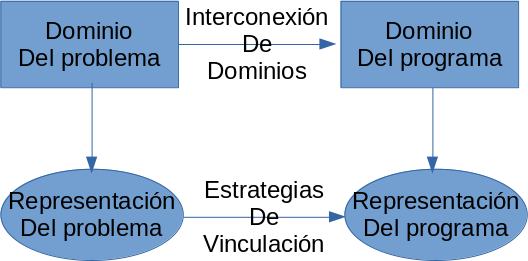
\includegraphics[width=6cm]{program_comprehension/domains.png}
    \centering
    \caption{Interrelación de Dominios}
\end{figure}

Existen diferentes estrategias\cite{BeronOliveiraCruz10} para este proceso de 
\textit{inter-relación de dominios}.
Los mismos son explicados brevemente a continuación:

\paragraph{SVS (Simultaneous Visualization Strategy)}
En esta estrategia, se utiliza información extraída dinámicamente, a través de
la instrumentación del código fuente.
Un inspector, insertado durante la instrumentación, extrae información de las funciones 
que son ejecutadas; mientras que el monitor se encarga de mostrar esta información.
De esta manera, mediante la ejecución y observación, el programador puede relacionar
el Dominio del Problema con el Dominio del Programa. 

\paragraph{BORS (Behavioral-Operational Relation Strategy)}
Al igual que la SVS, en esta estrategia también se utiliza instrumentación del código,
para extraer información del árbol de llamada de funciones.
Esta estrategia se plantea en tres pasos.
En el primero, de índole observacional, se identifican los objetos del dominio y sus interfaces,
los cuales a través de algunas técnicas son extraídos y puestos en una lista.
El segundo paso, a través de la ejecución del código ya instrumentado, construye el árbol de
llamadas.
El tercer y último paso, consiste en asociar el árbol de llamadas extraído en el segundo paso,
con el listado de interés definido en el primer paso.
Con este proceso, el programador puede relacionar y validar el comportamiento esperado del programa
con los elementos que lo ejecutan\cite{FonsecaCruzHenriquesPereira08}.

\paragraph{SVSi (Simultaneous Visualization Strategy Improved)}
Ambos enfoques anteriores presentan inconvenientes, los cuales son tratados de resolver
con esta estrategia.
SVS relaciona los dominios, pero carece de explicaciones; mientras que BORS puede proporcionarlas,
pero requiere intervención manual.
SVSi, utilizando la salida de SVS (funciones ejecutadas) como entrada para BORS, busca
suplir las falencias mencionadas.
